%Incidencia de una onda plana a 45° con n_i = 1, n_t = 1.46   

\documentclass[tikz,crop]{standalone}

\usepackage{tikz}
\usetikzlibrary{decorations.pathreplacing,decorations.pathmorphing}
\usepackage{physics}

\begin{document}


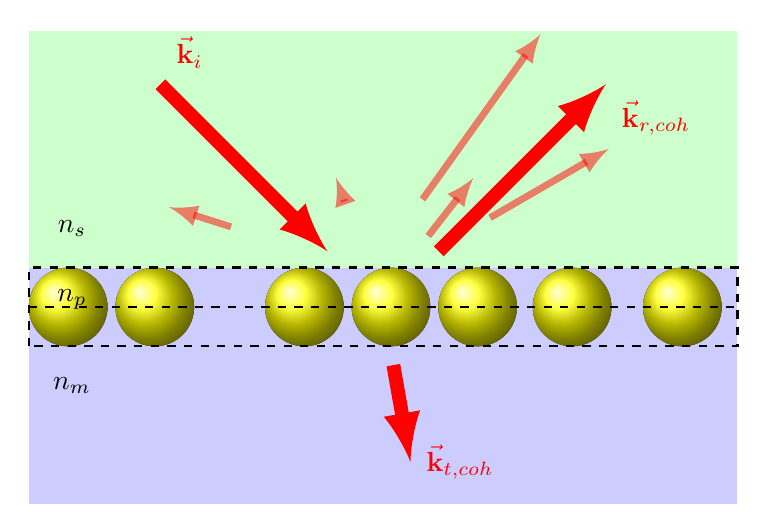
\begin{tikzpicture}%[   ESTO PONE LAS RAYAS QUE USO EN EPSEJOS
%    interface/.style={
        % The border decoration is a path replacing decorator. 
        % For the interface style we want to draw the original path.
        % The postaction option is therefore used to ensure that the
        % border decoration is drawn *after* the original path.
%        postaction={draw,decorate,decoration={border,angle=-45,
%                    amplitude=0.3cm,segment length=2mm}}},
%    ]



%-------------------------------------------- Incidence media


\def\a{.5}
\def\d{.5}

\fill[blue, opacity = .2] (-4.5,-2.5) rectangle(4.5,\d);
\fill[green, opacity = .2] (-4.5,\d) rectangle(4.5,3.5);

\foreach \x in {-4,-2.9,-1,.1,1.2,2.4,3.8}{
\fill[ball color=yellow, opacity=1] (\x,0) circle(\a);}


\draw[thick, dashed] (-4.5,0)--(4.5,0);
\draw[thick, dashed] (-4.5,-\d) rectangle (4.5,\d);

\draw[latex -, thick, red, line width=5](135:1)--(135:4) node[anchor=south west]{$\va{k}_i$};
\draw[- latex, thick, red, line width=5](45:1)--(45:4)node[anchor=north west]{$\va{k}_{r,coh}$};
\draw[- latex, thick, red, line width=5](-80:.75)--(-80:2)node[anchor=west ]{$\va{k}_{t,coh}$};

\begin{scope}[transparency group]
	\draw[- latex, red, opacity=.5,line width=2.5](0,\d)++(25:1.5)--(35:3.5);
	\draw[- latex, red, opacity=.5,line width=2.5](0,\d)++(35:.7)--(55:2);
	\draw[- latex, red, opacity=.5,line width=2.5](0,\d)++(165:2)--(155:3);
	\draw[- latex, red, opacity=.5,line width=2.5](0,\d)++(120:1)--(110:1.75);
	\draw[- latex, red, opacity=.5,line width=2.5](0,\d)++(60:1)--(60:4);
\end{scope}


\node at (-4,1) {$\; n_s$};
\node at (-4,.1) {$\; n_p$};
\node at (-4,-1) {$\; n_m$};

\end{tikzpicture}


\end{document}